%%%%%%%%%%%%%%%%%%%%%%%%%%%%%%%%%%%%%%%%%
% Dreuw & Deselaer's Poster
% LaTeX Template
% Version 1.0 (11/04/13)
%
% Created by:
% Philippe Dreuw and Thomas Deselaers
% http://www-i6.informatik.rwth-aachen.de/~dreuw/latexbeamerposter.php
%
% This template has been downloaded from:
% http://www.LaTeXTemplates.com
%
% License:
% CC BY-NC-SA 3.0 (http://creativecommons.org/licenses/by-nc-sa/3.0/)
%
%%%%%%%%%%%%%%%%%%%%%%%%%%%%%%%%%%%%%%%%%

%----------------------------------------------------------------------------------------
%	PACKAGES AND OTHER DOCUMENT CONFIGURATIONS
%----------------------------------------------------------------------------------------

\documentclass[final,hyperref={pdfpagelabels=false}]{beamer}

\usepackage[orientation=portrait,size=a0,scale=1.4]{beamerposter} % Use the beamerposter package for laying out the poster with a portrait orientation and an a0 paper size

\usetheme{I6pd2} % Use the I6pd2 theme supplied with this template

\usepackage[english]{babel} % English language/hyphenation

\usepackage{amsmath,amsthm,amssymb,latexsym} % For including math equations, theorems, symbols, etc

%\usepackage{times}\usefonttheme{professionalfonts}  % Uncomment to use Times as the main font
%\usefonttheme[onlymath]{serif} % Uncomment to use a Serif font within math environments

\boldmath % Use bold for everything within the math environment

\usepackage{booktabs} % Top and bottom rules for tables

\graphicspath{{figures/}} % Location of the graphics files

\usecaptiontemplate{\small\structure{\insertcaptionname~\insertcaptionnumber: }\insertcaption} % A fix for figure numbering


% Additional packages
\usepackage[misc]{ifsym}

% commands
\newcommand{\todo}[1]{\textcolor{red}{\{\textbf{#1}\}}}

%----------------------------------------------------------------------------------------
%	TITLE SECTION 
%----------------------------------------------------------------------------------------

\title{\huge The Intrinsic Manifolds of Radiological Images and their Role in Deep Learning} % Poster title

\author{Nicholas Konz\textsuperscript{1}\and Hanxue Gu\textsuperscript{1} \and Haoyu Dong\textsuperscript{2} \and Maciej Mazurowski\textsuperscript{1,2,3,4} } % Author(s)

\institute{\textsuperscript{1}Department of Electrical and Computer Engineering, \textsuperscript{2}Department of Radiology, \textsuperscript{3}Department of Computer Science, \textsuperscript{4}Department of Biostatistics \& Bioinformatics,\\Duke University, Durham, North Carolina, USA} % Institution(s)

%----------------------------------------------------------------------------------------
%	FOOTER TEXT
%----------------------------------------------------------------------------------------

\newcommand{\leftfoot}{http://www.LaTeXTemplates.com} % Left footer text

\newcommand{\rightfoot}{Poster identifier: W69} % Right footer text

%----------------------------------------------------------------------------------------

\begin{document}

\addtobeamertemplate{block end}{}{\vspace*{2ex}} % White space under blocks

\begin{frame}[t] % The whole poster is enclosed in one beamer frame

\begin{columns}[t] % The whole poster consists of two major columns, each of which can be subdivided further with another \begin{columns} block - the [t] argument aligns each column's content to the top

\begin{column}{.02\textwidth}\end{column} % Empty spacer column

\begin{column}{.47\textwidth} % The first column

\begin{block}{Introduction}

\begin{columns} % Subdivide the first main column
\begin{column}{.54\textwidth} % The first subdivided column within the first main column
\begin{itemize}
\item \textbf{The Manifold Hypothesis (MH)}: \textit{High dimensional data can be well described by a much smaller number of} \textbf{intrinsic dimensions}.
    \begin{itemize}
    %\item The intrinsic dimension of a dataset estimates its information content. 
    \item Neural networks can learn to convert raw data to abstract, informative features that are \textit{intrinsic} to the dataset. % \cite{ansuini2019intrinsic}.
    \end{itemize}

\end{itemize}
\end{column}

\begin{column}{.43\textwidth} % The second subdivided column within the first main column
\centering
\begin{figure}
    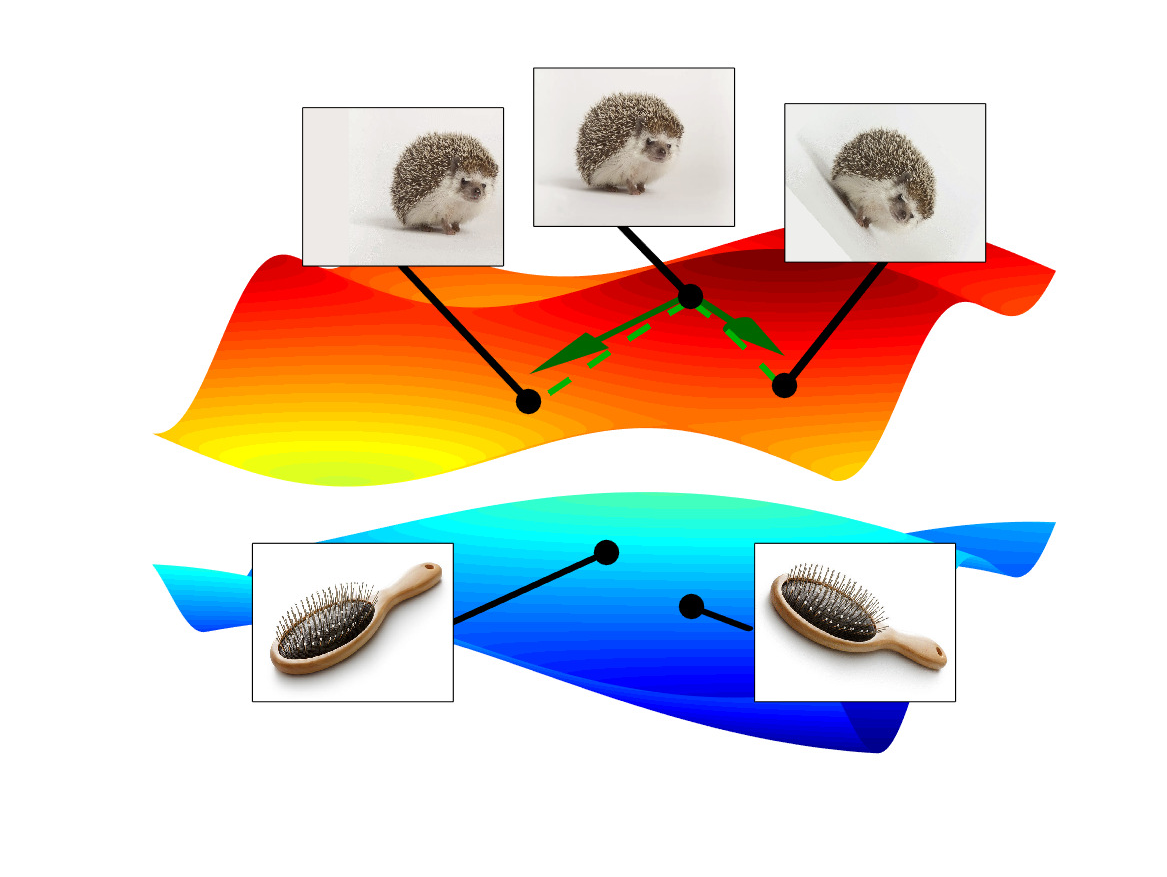
\includegraphics[width=0.8\linewidth]{buchanan_etal_fig1.pdf}
     \caption{\,Visualization of intrinsic low-dimensional image manifolds from \cite{buchanan2021deep}.}
\end{figure}
\end{column}
\end{columns} % End of the subdivision
\begin{itemize}
\item \textbf{Why study the intrinsic dimension of medical images?}
    \begin{itemize}
        \item Medical vs. natural images: different relevant semantics, 
        %yet we lack an understanding of how networks learn differently between the domains.
        \item Due to the MH, understanding the intrinsic structure of medical image datasets is key to analyzing how networks learn from them.
        %\item We can answer questions such as ``how does the intrinsic dimension of a dataset affect how challenging it is for a network to learn to generalize to new data from it?''
    \end{itemize}
\end{itemize}

\end{block}

\begin{block}{Objectives}

\begin{enumerate}
\item Estimate the intrinsic dimensions of common radiology datasets, and compare to natural image datasets.
\item Evaluate the relationship of dataset intrinsic dimension with network generalization ability; comparing within and between the domains of radiological and natural images.
\end{enumerate}

\end{block}

\begin{block}{Estimating the Intrinsic Dimension of Image Manifolds}
\begin{itemize}
    \item By the MH: our $d$-dimensional data lies on a manifold $\mathcal{M}\subseteq \mathbb{R}^d$ such that $\mathrm{dim}\,{\mathcal{M}}=m\ll d$.
\item We can estimate $m$ via \textbf{maximum likelihood}:
    \begin{itemize}
        \item Assume that volume of $\mathcal{M}$ scales exponentially with $m$ as we move away from a point; model volume with $k$-NN distance $T_k$.
        \item Model data sampling with a Poisson Process, and find $m$ via MLE:
        \begin{equation*}
            \label{eq:id_mle}
                \hat{m}=\left[\frac{1}{N(k-1)} \sum_{i=1}^{N} \sum_{j=1}^{k-1} \log \frac{T_{k}\left(x_{i}\right)}{T_{j}\left(x_{i}\right)}\right]^{-1}
        \end{equation*}
    \end{itemize}

\end{itemize}
\end{block}

\begin{block}{Datasets}

\begin{itemize}
\item 7 common radiology datasets from different modalities:
\end{itemize}
\begin{figure}
    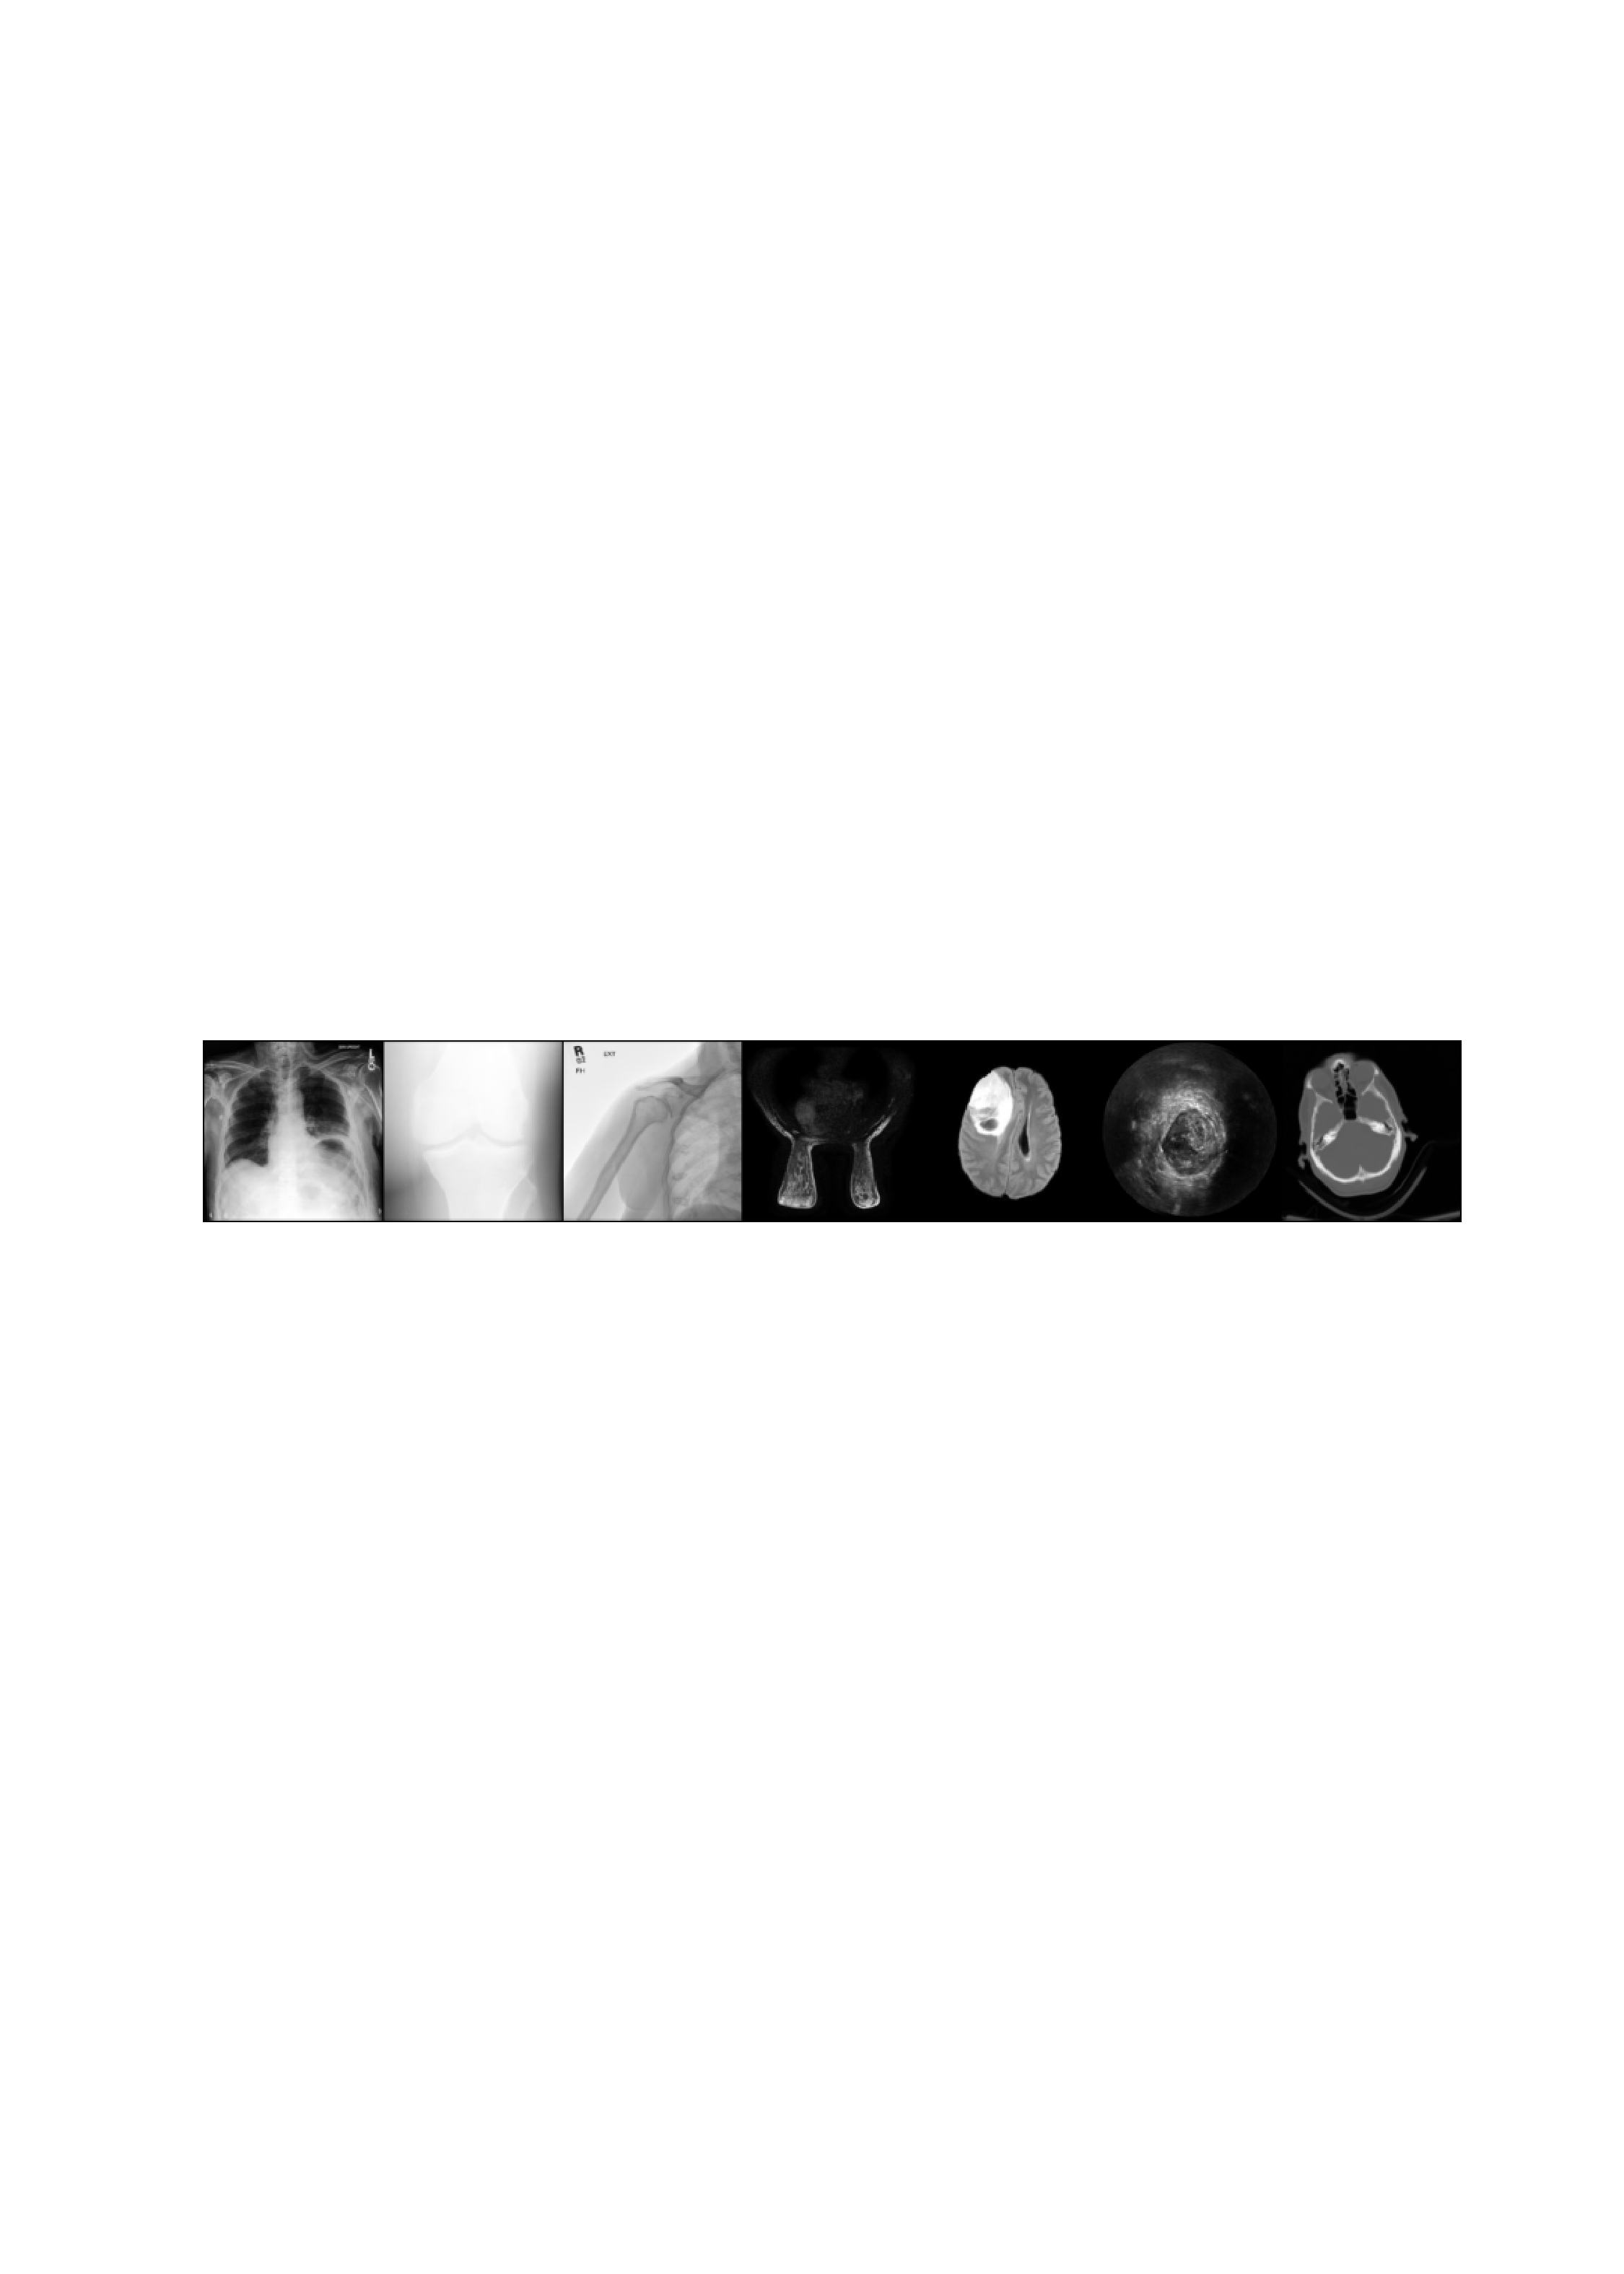
\includegraphics[width=0.95\linewidth]{frompaper/data_eg_1row.pdf}
    \caption{\,Samples from our seven evaluated datasets.}
\end{figure}

\end{block}


\setbeamercolor{block title}{fg=black,bg=paperblue!40} % Change the block title color
\setbeamercolor{block body}{fg=black,bg=paperblue!20} % Change the block title color
\begin{block}{Finding 1: Radiological vs. Natural Image Intrinsic Dimension}
    Radiological image datasets tend to have lower intrinsic dimension than natural image datasets:
    \begin{figure}
        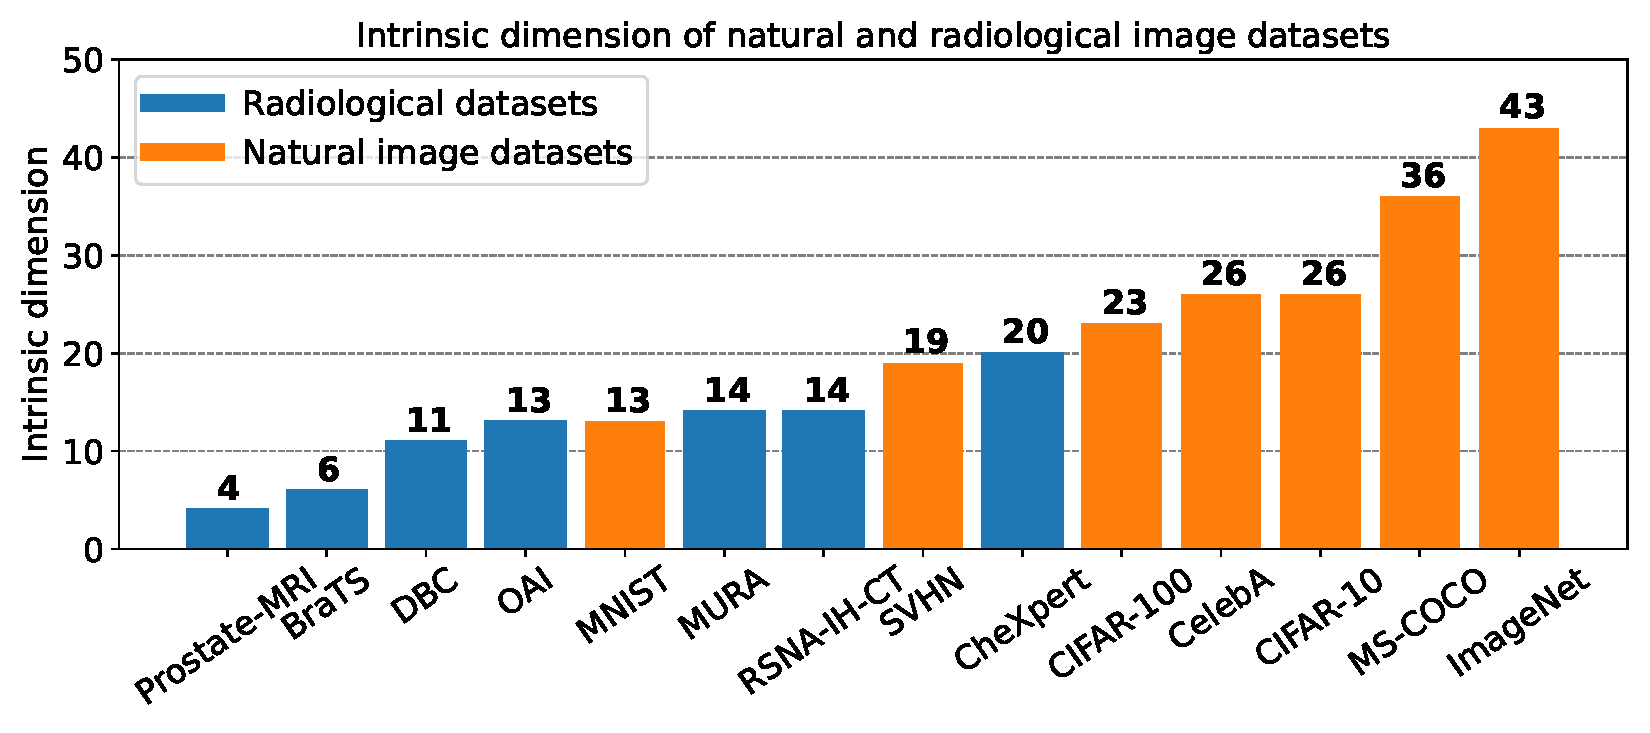
\includegraphics[width=0.95\linewidth]{frompaper/modified/ID.pdf}
        \caption{\,Intrinsic dimension of \textcolor{paperblue}{radiological} and \textcolor{paperorange}{natural} \cite{pope2021intrinsic} image datasets.}
    \end{figure}
\end{block}

%----------------------------------------------------------------------------------------

\end{column} % End of the first column
\begin{column}{.02\textwidth}\end{column} % Empty spacer column

 
\begin{column}{.47\textwidth} % The second column

%\begin{block}{Result 1: }
%\begin{itemize}
%    \item For each dataset, we estimate intrinsic dim using $7500$ images, evenly class-balanced according to a chosen binary classification task for each.
%\end{itemize}
%\end{block}



% \begin{itemize}
%     \item Additional findings:
%     \begin{itemize}
%         \item ID $\ll$ extrinsic dimension (ED/num. of pixels).
%         \item Intuitively, modifying ED (resizing images) didn't affect ID.
%     \end{itemize}
% \end{itemize}

% k}

\setbeamercolor{block title}{fg=black,bg=paperblue!40} % Change the block title color
\setbeamercolor{block body}{fg=black,bg=paperblue!20} % Change the block title color
\begin{block}{Finding 2: Intrinsic Dimension and Generalization Ability}
\begin{itemize}
    \item Generalization ability (GA) is sharply linearly correlated with dataset intrinsic dimension (ID) \textit{within} radiological and natural imaging domains, but the steepness of this correlation differs noticeably \textit{between} the two domains.
    \item The \textit{slope} of this GA vs. ID relationship is practically independent to model choice and/or training set size within an imaging domain.
    %\item Our data also supports existing predictions that GA $\sim\propto \log N_{train}$.
\end{itemize}
\begin{figure}
   \label{fig:linear}
   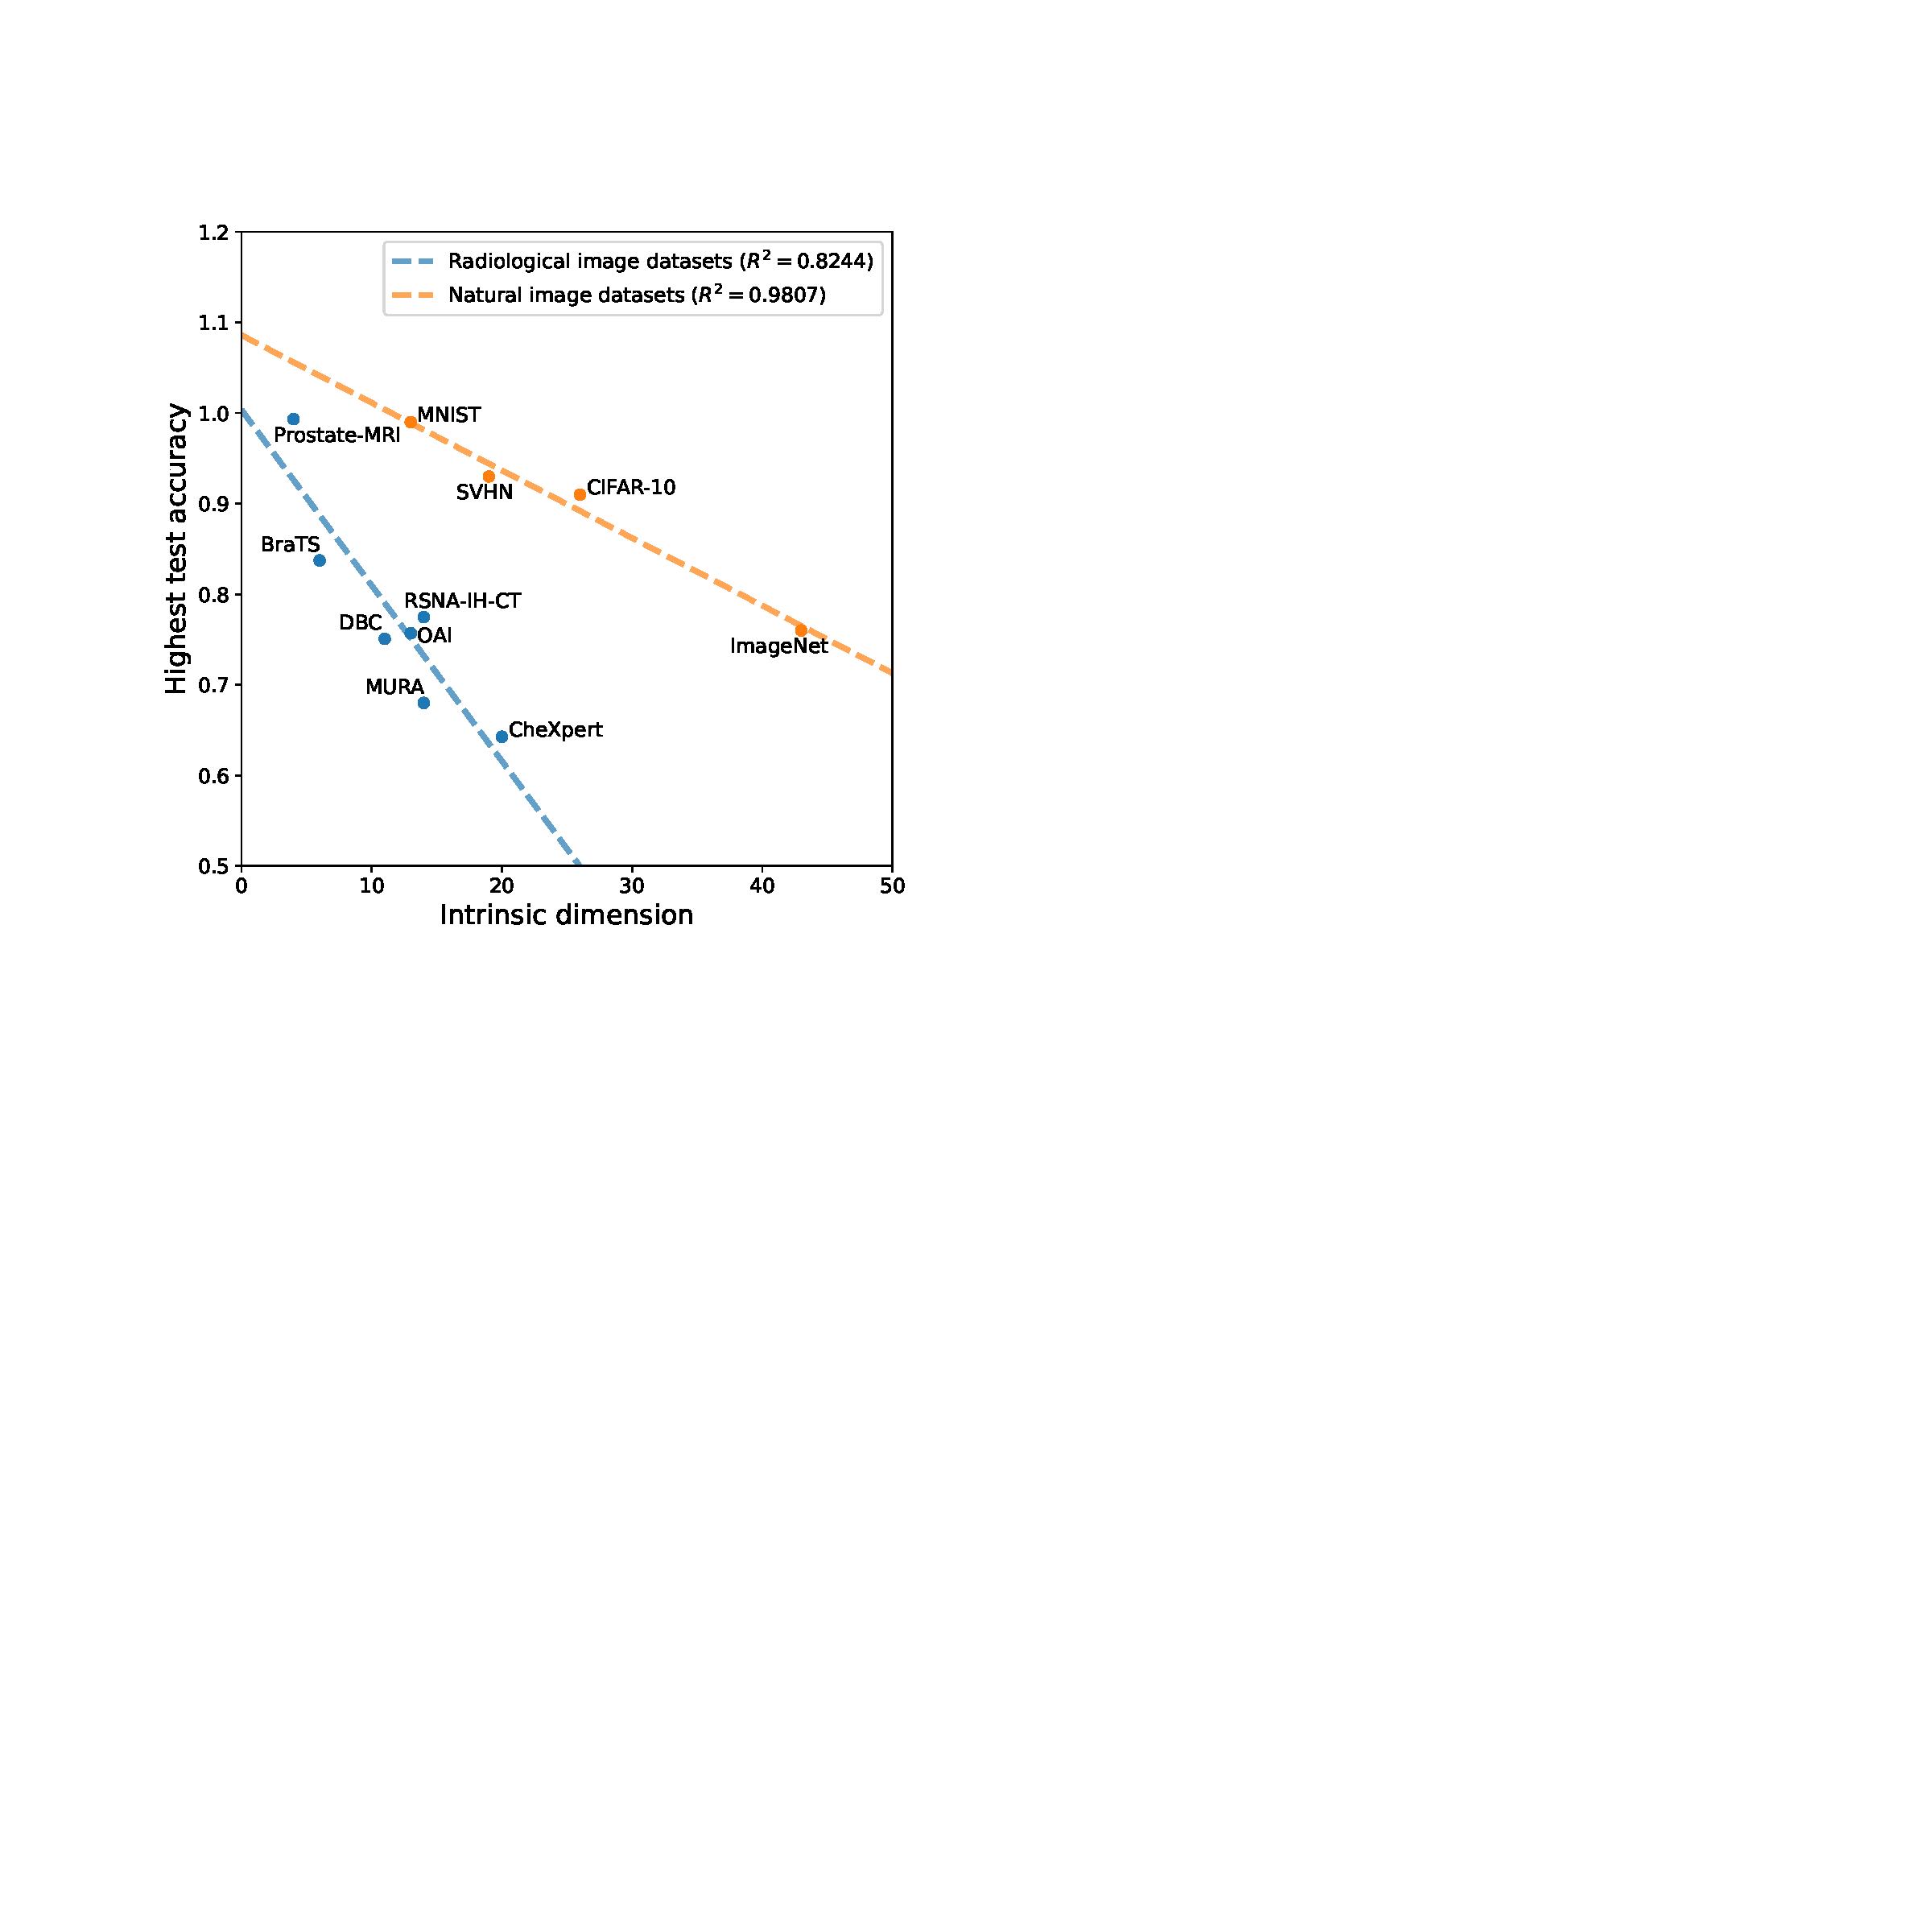
\includegraphics[width=0.75\linewidth]{frompaper/main_fig_multi_0.pdf}
   \caption{\,Linearity of model generalization ability with respect to dataset intrinsic dimension, for \textcolor{paperblue}{radiological} and \textcolor{paperorange}{natural} image datasets ($N_\text{train}=2000$ on ResNet-18).}
\end{figure}
\end{block}

\setbeamercolor{block title}{fg=black,bg=ta2aluminium} % Change the block title color
\setbeamercolor{block body}{fg=black,bg=white} % Change the block title color
% \begin{block}{Additional Findings}
%     \begin{itemize}
%         \item ID $\ll$ extrinsic dimension/ED (number of pixels).
%         \item Intuitively, modifying ED (resizing images) didn't affect ID.
%     \end{itemize}
% \end{block}
\begin{block}{Experimental Settings}
    \begin{itemize}
        \item \textbf{Radiological vs. natural image IDs (Finding 1):}
        \begin{itemize}
            \item We estimated the intrinsic dimension of each dataset using $7500$ images, evenly class-balanced according to a chosen binary classification task for each.
        \end{itemize}

        \item \textbf{Generalization ability vs. ID (Finding 2):}
        \begin{itemize}
        \item We trained a network on each dataset for its respective binary classification task, and tested on 750 unseen data points.
        \item We evaluated 9 neural network models, each on 7 training set sizes, also performing task choice ablations.
        \end{itemize}
    \end{itemize}

\end{block}

\begin{block}{Future Work}

\begin{itemize}
\item Find theoretical support for the correlation of GA with dataset ID, and explain why the correlation sharpness differs between domains.
\item Explore further uses of dataset ID estimation for modeling, experimentation, etc.
\end{itemize}

\end{block}

\setbeamercolor{block title}{fg=black,bg=orange!70} % Change the block title color
\setbeamercolor{block body}{fg=black,bg=orange!50} % Change the block title color
\begin{block}{Contact Information}
\begin{itemize}
\item My email: \href{mailto:nicholas.konz@duke.edu}{nicholas.konz@duke.edu}
\item My website: \url{https://nickk124.github.io/}
\item Lab website: \url{https://sites.duke.edu/mazurowski/}
\end{itemize}
\end{block}
\begin{block}{References}
        
% \nocite{*} % Insert publications even if they are not cited in the poster
\small{\bibliographystyle{unsrt}
\bibliography{mainbib}}

\end{block}
%----------------------------------------------------------------------------------------

\end{column} % End of the second column

\begin{column}{.02\textwidth}\end{column} % Empty spacer column
 
\end{columns} % End of all the columns in the poster

\end{frame} % End of the enclosing frame

\end{document}